\section{6LoWPAN}

\subsection{Routing (RPL)}

\begin{frame}{Routing in 6LoWPAN}{RPL}
		\begin{block}{}
			\begin{itemize}
			\item 	dynamisches Routing-Protokoll
					für energiearme und verlustbehaftete Netzwerke
			\item 	Route-Over-Protokoll
			\item 	Protokoll auf Basis eines Distanzvektor-Algorithmus:
					\begin{itemize}
					\item 	DODAG (Destination Oriented Directed Acyclic Graph)
					\item 	jeder Knoten besitzt einen Rang
					\item 	spezielle Nachrichten zum Austausch der
							Routing-Informationen \eg{(DIO, DIS, DAO)}
					\item 	Zielfunktion berechnet Rang
							und wählt bevorzugten Elternknoten
					\end{itemize}
			\item 	weitere Besonderheiten:
					\begin{itemize}
					\item 	Local und Global-Repair (z.B. bei Ausfall eines Knotens)
					\item 	Verwendung des Trickle Timer Algorithmus
					\end{itemize}
			\item 	Implementation in Contiki: ContikiRPL
					\begin{itemize}
					\item 	keine im Standard definierten Sicherheitsmechanismen implementiert
					\end{itemize}
			\end{itemize}
		\end{block}
\end{frame}

\begin{frame}{Routing in 6LoWPAN}{RPL}
	\begin{figure}
	\centering
	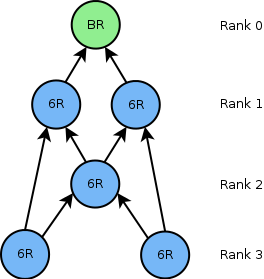
\includegraphics[width=0.5\linewidth]{Dodag}
	\linebreak
	\emph{Ein Beispielnetz}
	\end{figure}
\end{frame}
\subsection{Sensorknoten}

\begin{frame}{Sensorknoten letztes Semester}
	\begin{itemize}
	\item 	Sensor Terminal Board
			mit rcb128rfa1 Modul
	\item 	AVR ATmega128rfa1 Microcontroller
	\item 	Ansteuerung der Sensoren
			ohne Betriebssystem:
			\begin{itemize}
			\item 	Feuchtigkeitssensor
			\item 	Drucksensor
			\item 	Geschwindigkeitssensor
			\item 	Ansteuerung per I2C-Bus
			\end{itemize}
	\item 	Einarbeitung in Contiki:
			\begin{itemize}
			\item 	Wie können die Sensoren sinnvoll implementiert werden?
			\item 	Beachtung der Trennung von
					Core, CPU und Platform
			\item 	Nutzung bereits implementierter Schnittstellen
			\end{itemize}
	\end{itemize}
\end{frame}

\begin{frame}{Sensorknoten dieses Semester}
	\begin{itemize}
	\item 	deRFmega128-Board (Batteriebetrieb)
	\item 	AVR ATmega128rfa1 Microcontroller
	\item 	Verifizierung der I2C-Schnittstelle in Contiki durch neuen Sensor (Lichtsensor)
	\item 	Ansteuerung eines Aktors (Heizungsthermostat):
			\begin{itemize}
			\item 	zwei Boards, die per UART miteinander kommunizieren
			\item 	Software des Heizungsthermostat
					durch Bachelor-Projekt
					bereitgestellt
			\item 	das deRFmega128-Board stellt die Funk-Kommunikation bereit
			\end{itemize}
	\end{itemize}
\end{frame}

